\title{Group 10 Report: Rotten Potatoes} % Title
\author{郑时飞 \\ 朱伯源 \\ 李易 \\ 汪明杰 \\ 施天昊}% Author
\date{\today}% Date

\documentclass[11pt]{article}
\usepackage[margin=1in]{geometry}
\usepackage{vmargin}
\usepackage{url}
\usepackage{datetime}
\usepackage[utf8]{inputenc}
\usepackage{CJKutf8}
\usepackage{graphicx}
\usepackage{mathtools}
\usepackage{float}
\usepackage[colorlinks,linkcolor=blue,urlcolor=blue]{hyperref}


\makeatletter 
    \newcommand\fcaption{\def\@captype{table}\caption}
\makeatother
\setmarginsrb{3 cm}{2.5 cm}{3 cm}{2.5 cm}{1 cm}{1.5 cm}{1 cm}{1.5 cm}

\makeatletter
\let\thetitle\@title
\let\theauthor\@author
\let\thedate\@date
\makeatother

\usepackage{graphicx}
\graphicspath{{graphics/}}
\usepackage{geometry}
\geometry{left=5cm,top=5cm,right=0cm,bottom=0cm}

\usepackage[colorlinks,linkcolor=blue]{hyperref}

\begin{document}
\begin{CJK*}{UTF8}{gbsn}

\begin{titlepage}
    \centering
    \vspace*{0.5 cm}
    
\includegraphics[scale = 0.75,width=6cm]{CUHK}\\[1.0 cm]
    \textsc{\large The Chinese University of Hong Kong, Shenzhen}\\[1.5 cm] 
    \textsc{\Large CSC 3170}\\[0.5 cm] 
    \textsc{\large Database System}\\[0.5 cm]
    \rule{\linewidth}{0.2 mm} \\[0.4 cm]
    { \huge \bfseries \thetitle}\\
    \rule{\linewidth}{0.2 mm} \\[0.6 cm]
    
    \begin{minipage}{0.4\textwidth}
        \begin{flushleft} \large
            \emph{Authors:}\\
            郑时飞 \\ 朱伯源 \\ 李易 \\ 施天昊 \\ 汪明杰
            \end{flushleft}
    \end{minipage}~
    \begin{minipage}{0.4\textwidth}
            \begin{flushright} \large
            \emph{Student Number:} \\
            119010465 \\ 119010485 \\ 119010156 \\ 120090472 \\ 119010300
        \end{flushright}
    \end{minipage}\\[2 cm]
    {\large \thedate}\\[2 cm]
 
    \vfill
    
\end{titlepage}

\tableofcontents
\pagebreak

\rmfamily
\section{Introduction}
\paragraph{}As an art and commercial work, movies have become pursuits of many people and generated tremendous value. Currently, there are two types of online movie platforms. On the one hand, platforms including Rotten Tomatoes and Douban gives people rich information regarding movies. On the other hand, sites like Netflix offers precise, personalized recommendation to users. Such a recommendation strategy allows users to discover more films they enjoy and attracts more users to the platform.
\paragraph{}However, currently, no site combines the strengths of the mentioned movie sites. Besides, existing popular movie websites are full of quarrels and controversies from the perspective of the community environment. The movie recommendation sare influenced deeply by the advertising, not the quality of films. Therefore, to satisfy the real requirements of movie lovers, we build a movie database called \textbf{Rotten Potatoes}, based on which, users can talk about their reviews on the movie freely. It also offers plenty of searching functions and personalized recommendations from the platform. 
\paragraph{}We use python packages \textbf{\textit{Requests}}, \textbf{\textit{BeautifulSoup}} to obtain the required data from IMDB, store it in a MySQL database. Then we build our searching functions and personalized moive recommendations on those data. We also build a user-friendly web using \textbf{\textit{amis}} as the front end and \textbf{\textit{express}} as the back end.
\section{Design}
In this section, we focus on the design of Entity-Relationship Model, 
the reduction from ER diagram into relational schemas, constraint and index.

\subsection{Entity-Relationship Model}
As shown in the ER digram below, there are 6 entities and 5 relationships. 
\begin{figure}[h]
\centering
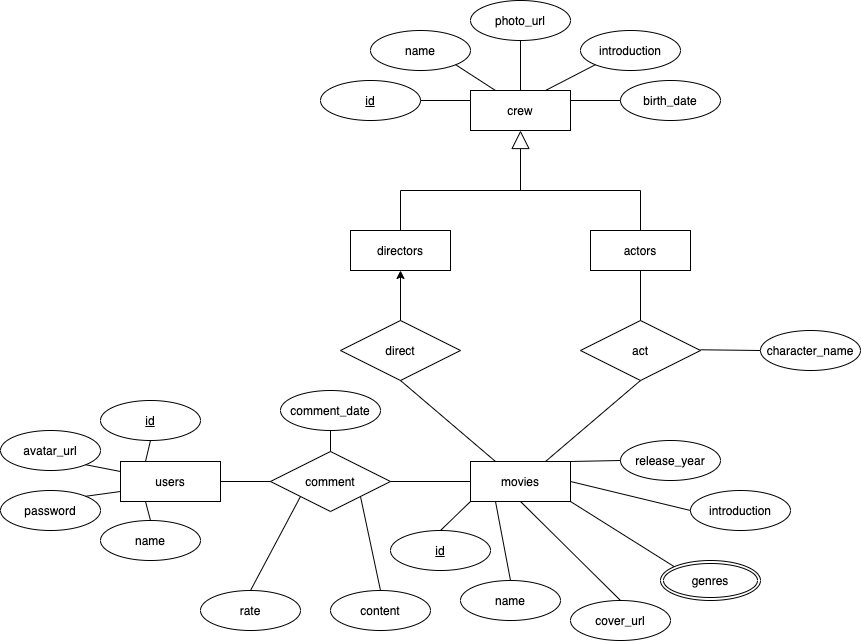
\includegraphics[width=0.8\textwidth]{er.png}
\caption{ER Diagram}
\end{figure}
\paragraph{Entity ``movies''}
To store id, name, cover url, introduction, release year and genres of a movie, where genres is a multivariate attribute. Identified by id. 
\paragraph{Entity ``directors''}
To store id, name, photo url, introduction and birth date of a director. This entity has a one-to-many relationship ``direct'' with the entity ``movies'', which means a director can directs multiple movies and a movie can be directed by only one director in our assumption. Identified by id. 
\paragraph{Entity ``actors''}
To store id, name, photo url, introduction and birth date of an actor. This entity has a many-to-many relationship with the entity ``movies'', which means an actor can act in multiple movies and a movie can be acted by multiple actors in our assumption. Identified by id. 
\paragraph{Entity ``users''}
To store id, name, avatar url, password of a user. This entity has a many-to-many relationship with the entity ``movies'', which means a user can comment on multiple movies and a movie can be commented by multiple users in our assumption. Identified by id. 
\paragraph{Entity ``characters''}
To store movie id (of the movie where this character appears), actor id (of the actor who acts as this character), id, character name of a character. This entity is a weak entity identified by entity ``movies'' through relationship ``appear'' and entity ``actors'' through relationship ``act as'', and also by its own id, which means a character can be acted by exactly one actor and appear in exactly one movie in our assumption (we treat characters of the same name appearing in multiple movies or acted by multiple actors as multiple different characters for simplicity). Note that since this entity is also identified by its own id, it is allowed that an actor acts as multiple characters in the same movie. 
\paragraph{Entity ``comments''}
To store movie id (of the movie commented by this comment), user id (of the user who makes this comment), id, rate (from 0 to 10), content and comment date of a comment. This entity is a weak entity identified by entity ``movies'' and entity ``users'', and also by its own id, which means a comment is on exactly one movie and is made by exactly one user in our assumption. Note that since this entity is also identified by its own id, it is allowed that a user makes multiple comments on the same movie. 

\subsection{Relational Schema}
As shown in the relational schema digram below, there are 7 schemas. 
\begin{figure}[h]
\centering
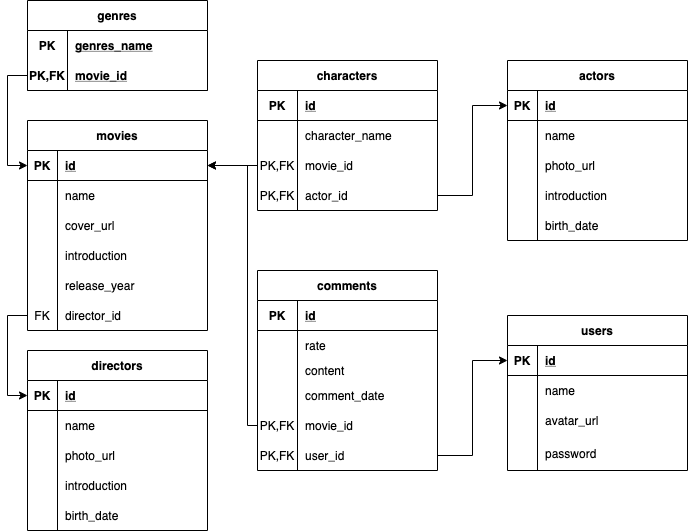
\includegraphics[width=0.8\textwidth]{schema.png}
\caption{Relational Schema Diagram}
\end{figure}

The following reductions are made:
\begin{itemize}
\item The attribute ``genres'' in entity ``movies'' is reduced to schema ``genres'' with attributes ``genres\_name'' and ``movie\_id'' as a foreign key, both of which forms a primary key to make sure no redundant genres of a movie.
\item The relationship ``direct'' between entity ``movies'' and ``directors'' is reduced to attribute ``director\_id''as a foreign key in schema ``movies'' so that a movie is directed by exactly one director. 
\item All attributes identifying the entity are reduced to primary keys.
\item ``movie\_id'', ``actor\_id'' of entity ``characters'', ``movie\_id'', ``user\_id'' of entity ``comments'' are reduced to foreign keys in their schemas referencing their corresponding identifying strong entities. 
\end{itemize}

\subsection{Constraint}
3 types of constraints are further added:
\paragraph{Not Null Constraints}
\begin{itemize}
\item All ``id'' attributes as they are primary key and thus automatically becoming not null.
\item ``name'' attribute of schema ``movies''.
\item ``name'' and ``director\_id'' attributes of schema ``directors'', as a movie is directed by exactly one director.
\item ``name'' attribute of schema ``actors''.
\item ``name'' and ``password'' attributes of schema ``users''.
\item ``actor\_id'', ``movie\_id'' and ``character\_name'' attributes of schema ``characters'', as it is a weak entity of schemas ``actors'' and ``movies''.
\item ``user\_id'', ``movie\_id'', ``rate'', ``content'' and ``comment\_date'' attributes of schema ``comments'', as it is a weak entity of schemas ``users'' and ``movies''.
\item ``genres\_name'', ``movie\_id'' attributes of schema ``genres'', as it is a multivariate attribute of schema ``movies''.
\end{itemize}
\paragraph{Unique Constraint}
A unique constraint is added to ``name'' attribute of schema ``users'' as by our assumption there should be no repeating user names. 
\paragraph{Check Constraint}
A check constraint is added to ``rate'' attribute of schema ``comments'' to make sure the rate is from 0 to 10.

\subsection{Index}
The following attributes are indexed to make search faster:
\begin{itemize}
\item ``name'' and ``release\_year'' attributes of schema ``movies''.
\item ``name'' and ``birth\_date'' attributes of schema ``directors''.
\item ``name'' and ``birth\_date'' attributes of schema ``actors''.
\item ``name'' attribute of schema ``users''.
\end{itemize}

\section{Implementation}
\subsection{Frontend}
\subsection{Backend}
\subsection{Web Crawler}
\subsection{Data Analysis}

\section{Result}

\section{Conclusion}
\paragraph{} In this project we build a moive database based on a large amount of data collected from \textbf{IMDB}. Additional attention is paid to assure a \textbf{BCNF} form is kept for every entity in our database, thus the redundancy part is eliminated. We also \textbf{implement useful functions} for our users to search for moives, casts or other users using name,  time information, rate(only moives) and genres(only moives) as the keyword.
\paragraph{} In order to improve user experience and replace the complex database operations by a few simple mouse clicks from users, we build a user friendly website. Based on that, abundant \textbf{personalized interaction behaviors} can be achieved, which serves our users more conviently. We hold an integral process of account management for users. Users can add comments to a moive and rate on it as well as discover their approbated reviews or users.
\paragraph{} It is common for a moive database to recommend moives that the users have potential interest in. However,  how to make a personalized recommendation lists of high quality is always a problem. We use a lot of techinques in the data analysis to satisfy the needs from users . We build a \textbf{Restricted Boltzmann Machines}  with \textbf{Neighbourhood model} and get gratifying results.
\section{Self-Evaluation}

\section{Contribution}

\end{CJK*}
\end{document}
